\section{Durchführung}
\label{sec:Durchführung}
Der Aufbau wird in \autoref{fig:Abb_2} dargestellt, wobei der He-Ne-Laser nict um die Strahachse schwenkbar ist.
\begin{figure}[H]
    \centering
    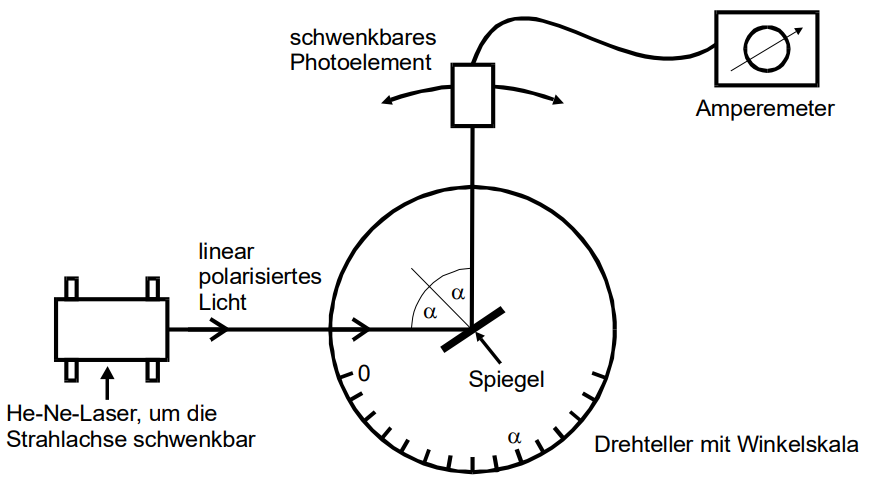
\includegraphics[width=0.5\textwidth]{Abbildung/Abb_2.png}
    \caption {Schematische Darstellung der verwendeten Messapparatur \cite{V407}.}
    \label{fig:Abb_2}
\end{figure}
Vor der eigentlichen Messung muss die Messappartur richtig justiert werden. Dazu wird der 
Silizium-Spiegel entfernt und eine Messung der Intensität des Laser-Strahls durchgeführt.
Anschließend wird der Spiegel auf den Probenhalter montiert und so kallibriet, dass der Laserstrahl
direkt auf den Laserkopf zurück reflektiert wird. Das Ginometer wird in dieser 
Stellung auf $\qty{0}{\degree}$ zeigt. Die Messung kann nun begonnen werden.\\
Für die eigentliche Messung wird ein Winkel für die Polarisation eingestellt.
Es werden die Polarisationswinkel $\qty{0}{\degree}$ und $\qty{90}{\degree}$  eingestellt.
Anschließend wird die Intensität des reflektierten Laserstrahls für unteschiedliche Eintrttswinkel gemessen und 
in eine Tabelle eingetragen. Das Winkelintervall ist von $\qty{4}{\degree}$ bis $\qty{87}{\degree}$.
Dabei werden die Messwerte in einem Abstand von $\qty{2}{\degree}$ aufgenommen.